\chapter{Friedmann-Gleichung\label{chapter:thema}}
\lhead{Friedmann-Gleichung}
\begin{refsection}
\chapterauthor{Andri Hartmann und Tobias Schuler}
\printbibliography[heading=subbibliography]
\section{Expansion des Universums}
Seit langem stellte man sich die Frage, was das Universum ist und wie es sich verhält. Als 1912 Albert Einstein die Relativitätstheorie herleitete, konnten gewisse Fragen beantwortet werden.
%\subsection{Kosmologische Rotverschiebung}
%Die Kosmologische Rotverschiebung ist nicht zu verwechseln mit dem Dopplereffekt. Grund daf\"{u}r ist, dass sich die Galaxien nicht in der Raumzeit voneinander entfernen, sondern sich der Raum ausdehnt. 
\subsection{Alexander Friedmann und Georges Lema\^{i}tre}
Beide entdeckten im Jahre 1927 unabhängig voneinander die Friedmann-Lema\^{i}tre-Gleichung. Diese beschreibt das Verhalten des Universums seit dem Urknall. 
\begin{equation}
\left(\frac{\dot{a}}{a}\right) ^2 = \frac{8 \pi G}{3} \rho - \frac{k c^2}{a^2} + \frac{\Lambda c^2}{3}
\end{equation}
\subsubsection{Herleitung der Gleichung}
Um an das Problem heranzugehen führen wir ein Koordinatensystem ein, welches sich mit der relativen Bewegung der Galaxien mitbewegt. Somit sind die Galaxien wie in einem Raster eingefroren. Die Einheit des Rasters wird durch den Skalenfaktor $a$ ausgedrückt und ist eine Funktion der Zeit. Verändert sich das Raster, verändern sich auch die Positionen der Sterne und Galaxien.
%\begin{figure}
%	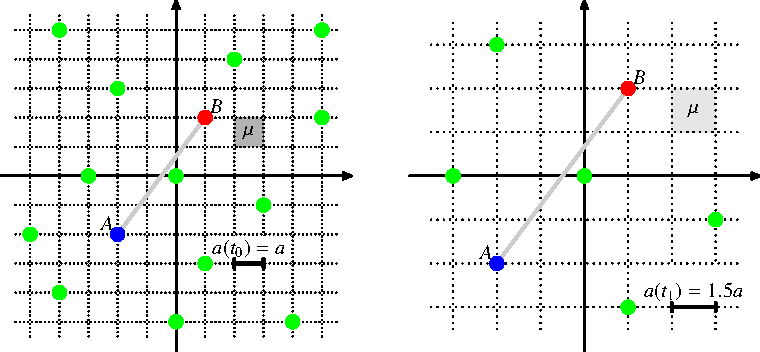
\includegraphics[width = \textwidth ]{chapters/images/friedmann-1.png}
%\end{figure}
Die Distanz zwischen zwei Punkten A und B entspricht 
\begin{equation}
D_{AB} = \sqrt{a^2(t)\Delta_{AB}x^2 + a^2(t)\Delta_{AB}y^2 + a^2(t)\Delta_{AB}z^2} = a(t) \sqrt{\Delta_{AB}x^2 + \Delta_{AB}y^2 + \Delta_{AB}z^2}
\end{equation}
F\"{u}r die Geschwindigkeit, mit der sich die beiden Punkte relativ zueinander bewegen, gilt 
\begin{equation}
v_{AB} = \dfrac{dD_{ab}}{dt} 
	   = \dot{a} \sqrt{\Delta_{AB}x^2 + \Delta_{AB}y^2 + \Delta_{AB}z^2}
\end{equation}
Um nun Aussagen über die Dynamik des Universums zu machen, die nicht von der fiktiven Wahl  des Skalenfaktors abhängen, teilen wir die Geschwindigkeit durch den Skalenfaktor $a$.
\begin{equation}
\frac{v_{AB} }{D_{AB}} = \frac{\dot{a}}{a}
\label{friedmann:geschwindigkeit}
\end{equation}
\begin{satz} [Hubble-Konstante]
	Die Ableitung des Skalenfaktors dividiert durch den Skalenfaktor entspricht der Hubble-Konstante.
	\[
	\frac{\dot{a}}{a} = H
	\]
\end{satz}
Das kosmologische Prinzip besagt, dass das Universum isotrop und homogen ist. Die Masse in einem Würfel mit Dimension $\Delta x$, $\Delta y$ und $\Delta z$ ist somit
\begin{equation}
M_{xyz} = \nu \Delta x \Delta y \Delta z
\end{equation}
Der Parameter $\nu$ beschreibt die Masse in einem Einheitsquadrant und ist somit von der Wahl von $a$ abhängig, jedoch konstant über die Zeit. Das Volumen des Würfels ist bekanntlich 
\begin{equation}
V_{xyz} = a^3 \Delta x \Delta y \Delta z
\end{equation}
und folglich kann die Massendichte geschrieben werden als
\begin{equation}
\rho = \frac{M_{xyz}}{V_{xyz}} = \frac{\nu}{a^3}
\label{friedmann:dichte}
\end{equation}
\subsubsection{Beschleunigung des Skalenfaktors}
Um die relative Beschleunigung zweier Punkte im Universum zu beschreiben, wird von folgendem Ansatz ausgegangen: Ein Beobachter befindet sich im Ursprung des Koordinatensystems und ist in Ruhe. Um nun die Kraft auf einen Körper der \textbf{Masse} $m$ im \textbf{Abstand} $D$ zu berechnen, denkt man sich eine Kugelschale um den Ursprung mit \textbf{Radius} $D$. Die Kraft auf den Körper verhält sich wie die Punktmasse aller  einzelnen Körper in der Kugel im Ursprung gedacht.
Für \textbf{Abstand} \textit{D}, \textbf{Geschwindigkeit} \textit{v} und \textbf{Beschleunigung} \textit{A} schreiben wir:
\[D =  a \sqrt{\Delta x^2 + \Delta y^2 + \Delta z^2}  = a R\]
\[v = \dot{a} R\]
\[A = \ddot{a} R\]

und für das Volumen V der Kugel
\[V = \frac{4 \pi }{3} a^3 R^3\]

Gemäss Newton ergibt sich die Gravitationskraft aus
\begin{equation}
F_G = -\frac{m M G}{D^2}
\end{equation}
Da die Gravitationskraft zwecks Vereinfachung des Modells als einzige Kraft eingesehen wird, gilt für die Beschleunigung mit 
\[F = m A\]
\[A = - \frac{M G}{D^2} = \ddot{a} R \Rightarrow \ddot{a} = \frac{- M G}{a^2 R^3} \Rightarrow\ \frac{\ddot{a}}{a} = \frac{-\frac{4 \pi }{3} M G}{\frac{4 \pi}{3}a^3 R^3} \Rightarrow \frac{\ddot{a}}{a} = \frac{- 4 \pi G}{3} \frac{M}{V}\]
Die Gleichung wurde so angepasst, dass oben die Masse und unten das Volumen steht. Damit vereinfacht sich die Beschleunigung zu
\begin{equation}
\frac{\ddot{a}}{a} = \frac{- 4 \pi G}{3} \rho
\end{equation}
\subsubsection{Bedeutung der Beschleunigungsgleichung}
Setzt man für die Dichte Gleichung \ref{friedmann:dichte} ein ergibt sich
\[\frac{\ddot{a}}{a} = \frac{- 4 \pi G}{3} \frac{\nu}{a^3} \Rightarrow \frac{\ddot{a}}{a} = \frac{- 4 \pi G \nu}{3} \frac{1}{a^3}\]
Durch geschickte Wahl des Skalenfaktors kann $\nu$ den konstanten Term auf der rechten Seite gegen 1 streben lassen. So vereinfacht sich die Gleichung zu
\[\frac{\ddot{a}}{a} = \frac{-1}{a^3} \Rightarrow \ddot{a} = \frac{-1}{a^2}\]
Die Differentialgleichung ist nichtlinear und mit MatLab nicht lösbar. Trotzdem können wir gewisse Aussagen machen, nämlich
\begin{enumerate}
	\item Die negative Beschleunigung wirkt der Ausdehnung des Universums entgegen. 
	\item Statisches Universum ist nicht möglich für $\rho \neq 0$.
	\item Die Formel hängt nicht vom Ort R ab, was bedeutet das unser Ansatz mit dem Beobachter im Ursprung legitim war.
\end{enumerate}

\subsubsection{Energieerhaltung}
Da wir versuchen, das Universum als ein physikalisches System zu beschreiben, muss auch hier der bedeutsame Satz der Energieerhaltung gelten. Im folgenden betrachten wir die radiale Ausdehnung des Universums aus einem Ursprung heraus (BIG BANG). Das Universum kann bei der Entstehung mit verschiedenen Gesamtenergien initialisiert werden, abhängig von der Dichte der Materie und ihrer Fluchtgeschwindigkeit.\\
Betrachten wir für den Anfang die Beziehung zwischen kinetischer und potentieller Energie.
\begin{equation}
E_{ges} = E_{kin} - E_{pot} =  \frac{m v^2}{2} - \frac{m M G }{x}, \qquad x = \text{Abstand zwischen der Masse M und m}
\end{equation}
Wir werden später noch andere Formen von Energie kennenlernen, die wir dieser Gleichung hinzufügen müssen. Doch beginnen wir in kleinen Schritten.\\
Die Gesamtenergie kann nun drei wesentliche, für die Dynamik interessante Werte annehmen,nämlich
\begin{enumerate}
	\item $E_{ges} > 0 \rightarrow$ Eine Masse $m$ entflieht der Schwerkraft.
	\item $E_{ges} = 0 \rightarrow$ Eine Masse $m$ nähert sich asymptotisch  der Geschwindigkeit null, bleibt aber nie stehen. (Fluchtgeschwindigkeit)
	\item $E_{ges} < 0 \rightarrow$ Eine Masse $m$ wird so stark angezogen, dass die Geschwindigkeit ihre Richtung ändert.
\end{enumerate}
Nennen wir die Gesamtenergie eine Konstante \textit{c} und formen die Gleichung um.
\[\frac{m v^2}{2} - \frac{m M G}{x} = c_1 \qquad| *\frac{2}{m} \qquad \]
\[{v^2} - \frac{2 M G}{x} = \frac{2c_1}{m} = c_2
\:  \Rightarrow \: \left( \dot{a} R\right)^2 = \frac{2 M G}{a R} + c_2\] 
\[\frac{\dot{a}^2}{a^2} = \frac{2 M G}{a^3 R^3} + \frac{c_2}{a^2 R^2} \: \Rightarrow \: \left(\frac{\dot{a}}{a} \right)^2 = \frac{\frac{4 \pi}{3}2 M G}{\frac{4 \pi}{3} a^3 R^3} + \frac{c_2}{a^2 R^2} \] %Schritte einzeln auflisten
Auf der rechten Seite der Gleichung erscheint jetzt die Masse der Kugel mit Radius $R$ und das Kugelvolumen $V$. Es gilt wieder Gleichung \ref{friedmann:dichte}. Daraus resultiert die vereinfachte Differentialgleichung 
\begin{equation}
\left(\frac{\dot{a}}{a} \right)^2 = \frac{8 \pi G}{3} \rho + \frac{c_2}{a^2 R^2}
\end{equation}
Mit \[\rho = \frac{\nu}{a^3}\]
\begin{equation}
\left(\frac{\dot{a}}{a} \right)^2 = \frac{8 \pi G}{3} \frac{\nu}{a^3} + \frac{c_2}{a^2 R^2}
\end{equation}
Vereinfacht
\begin{equation}
\left(\frac{\dot{a}}{a} \right)^2 = \frac{1}{a^3} + \frac{c}{a^2}
\end{equation}

\subsubsection{Diskussion der Differentialgleichung}
Wir erinnern uns, die Konstante \textit{c} steht für die Gesamtenergie des Universums und kann positiv, negativ oder null sein.
\begin{enumerate}
	\item Beginnen wir mit dem einfachsten Fall und setzen $c = 0$.
	\[\left(\frac{\dot{a}}{a} \right)^2 = \frac{1}{a^3}\]
	Um die Gleichung zu lösen, ziehen wir die Quadratwurzel und multiplizieren mit $a$.
	\[ \dot{a} = \frac{1}{\sqrt{a}} \]
	\[\frac{da}{dt} =\frac{1}{\sqrt{a}} \Rightarrow \frac{dt}{da} = \sqrt{a} \]
	\[ t = \frac{2}{3} a^{3/2} \Rightarrow a = \frac{3}{2} t^{2/3} \]
	Wir vernachlässigen der Vorfaktor und schreiben das wichtige Resultat
	\begin{equation}
	a = t^{2/3}
	\end{equation}
	
	\item Für den zweiten Fall ist $c > 0$.
	\[\ \left(\frac{\dot{a}}{a} \right)^2 = \frac{1}{a^3} + \frac{c}{a^2}\]
	Betrachten wir die rechte Seite, bemerken wir den Potenzunterschied im Nenner. Daraus folgt, dass für \textbf{kleine} \textit{a's} der \textbf{erste} Term dominiert, während der \textbf{zweite} Term für \textbf{grosse} \textit{a's} dominiert. Das kleine Universum verhält sich also wie für $c = 0$. Für ein grosses \textit{a} schreiben wir
	\[\ \left(\frac{\dot{a}}{a} \right)^2 = \frac{c}{a^2} \: \Rightarrow \:	\dot{a}^2 = c \: \Rightarrow \: \dot{a} = \sqrt{c_1} = c_2\]
	\begin{equation}
	a = c*t
	\end{equation}
	
	\item Als letztes soll $c < 0$ sein
	\[\ \left(\frac{\dot{a}}{a} \right)^2 = \frac{1}{a^3} - \frac{|c|}{a^2} \: \Rightarrow \: \dot{a}^2 = \frac{1}{a} - |c|\]
	\begin{equation}
	\dot{a} = \pm \sqrt{\frac{1}{a} - |c|}
	\end{equation}
	Anhand des Phasendiagramms erkennt man die Lösung dieser Differentialgleichung. Es beschreibt ein in sich zusammenfallendes Universum, auch Big-Crunch genannt.
	
\end{enumerate}

\begin{figure}
	\centering
	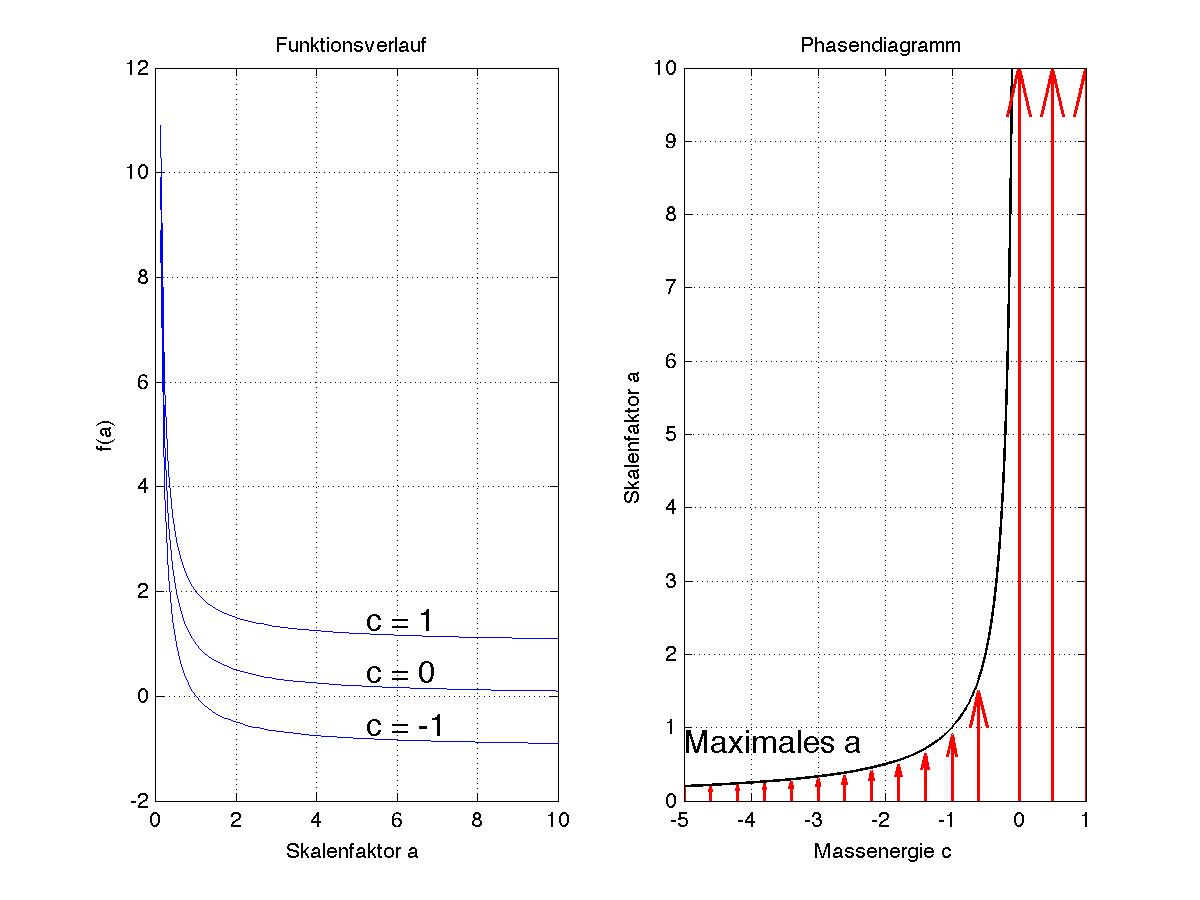
\includegraphics[width  = \textwidth]{chapters/images/phasendiagramm.jpg}
	\caption{Phasenportrait in Abhängigkeit der Gesamtenergie c
		\label{friedmann:phasenportrait}}
\end{figure}%


\begin{figure}
	\centering
	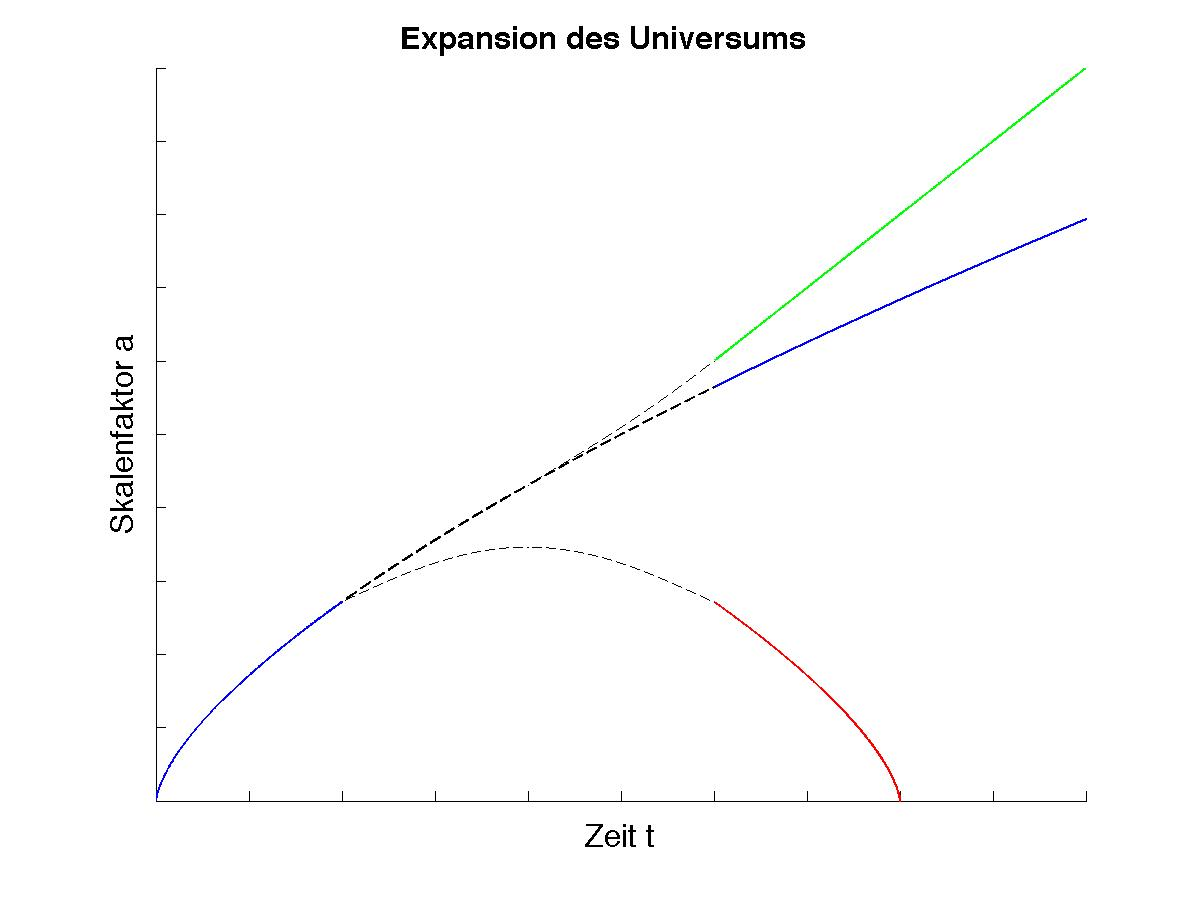
\includegraphics[width  = \textwidth]{chapters/images/friedmannGleichung.jpg}
	\caption{Verhalten des Universums in Abhängigkeit von der Zeit $t$
		\label{friedmann:friedmannGleichung}}
\end{figure}%

\subsection{Redshift}
Es stellt sich die Frage, wie sich die momentane Ausbreitungsgeschwindigkeit feststellen lässt. Dabei nutzt man die Erkenntnis, dass sich die Wellenlänge von Licht, welches sich durch einen ausdehnenden Raum bewegt, mit dehnt und somit ein anderes Farbspektrum erhält. Diese Verschiebung der Wellenlänge ins Rot nennt man in der Kosmologie Rotverschiebung. Daraus kann man nun die Ausdehnung des Raums während der Zeit, die das Licht reist, ausrechnen.
	
\end{refsection}
